\chapter{\uppercase{Location Prediction}}

Based on the questions we answered in the previous section, we have enough
information to build a system for location prediction, which we call
FriendlyLocation.
Since the location prediction system will be run on a large number of of users,
it must be fast and scalable.

\section{Edge Length Prediction}

Before we predict a user's location, we need a way to estimate the probabilty
that a geo-located user is at a location given the position of their contact.
%
To achieve this, we trained a regression tree to predict the distance between a
user and a contact.
%
The regreession tree was trained on several of the features from the previous
section that are correlated with users living near each other:
\begin{itemize}
\item the type of contact
\item if the geo-located user mentioned the contact
\item if the contact had a protected account
\item the contact's follower count
\item the quality of the contacts's locatation
\item the contact's local contact ratio
\end{itemize}
%
Since the distances between users varied by several orders of magnitude, we
trained the regreessor to predict the log of the distnace.
%
The tree regressor was configured to not split leafs with fewer than 1000 data
points to prevent over-fitting.
% FIXME: this needs more, but I'm not sure what.


\section{Model}
\label{sec:model}

In this section, we build a model for the probability that a user, who we refer
to as the target user, lives at a specific location given the approximate
location of his contacts.
%
In the previous sections, we looked at the probability that a contact lived a
certain distance from a given user.
%
Location prediction requires the probability that the user lives at a specific
location.


\begin{figure}[tb]
\centering
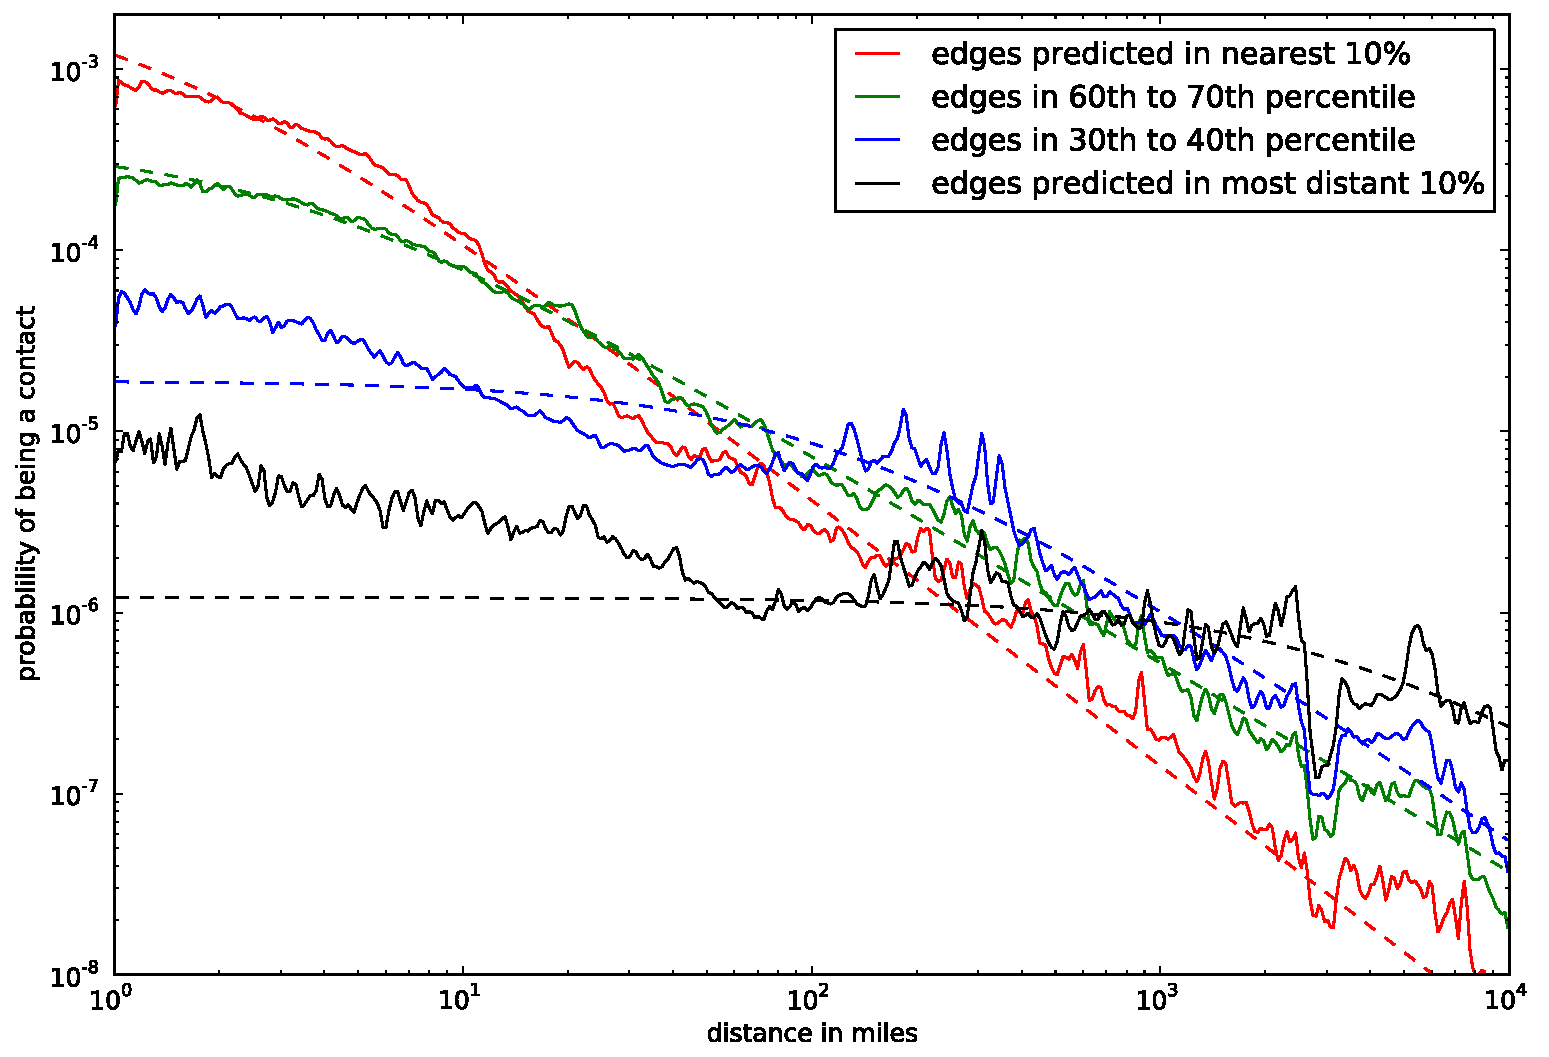
\includegraphics[width=\linewidth]{figures/near_prob_fit.pdf}
\caption{
After splitting edges into groups based their predicted distance, each group was fit to a curve. Here are four sample curves.
}
\label{fig:NearProbFit}
\end{figure}


% Put more about fit_stgrs
The edges were sorted by the distance that the tree regressor predicted and
split into ten equal groups.
%
For each of these groups, we calculated the distance to friends and fit it to
the curve a(b+x)**-c .
%
Four of the ten curves and their lines of best fit are shown in
Figure~\ref{fig:NearProbFit}. The best contacts are orders of magnitude more
likely to live near a target user than the worst contacts.
%
If the predictions from the tree regressor were ignored, and users were placed
into one group instead of ten equal groups, this would reduce to the model
for freindship and distance presented in \cite{backstrom2010find}.

FIXME: add details here.
FIXME: edge distance prediction

\section{System}
We used this model to build a Maximum Likelihood Estimator.
FriendlyLocation trained on FIXME edges from users in the training set to
their contacts.

FIXME: describe this

We use this to create a simple procedure for estimating the location for a user:
\begin{enumerate}
\item Pick up to 25 of the user's contacts.
\item Geocode the location field and calculate the the predicted error for each
of the contacts.
\item Ignore any contacts who have no decodable location information.
Approximately one third of the contacts are ignored.
\item For each of the contacts' locations calculate the probability that the
target user lives there using the maximum likelihood estimator.
\item Pick the location with the highest probability.
\end{enumerate}

FIXME: lots more here

